\section{Genetische Algorithmen}
% Wie Spielen diversifizierung und intensivierung mit ein?
% - Beim erstellen der initialen Population sollte man eine hohe Diversität anstreben, da es sonst zu einer verfrühten konvergenz kommen kann.
\textbf{Evolutionäre Algorithmen} sind stochastische populationsbasierte Metaheuristiken, welche dem Prozess der natürlichen Selektion nachempfunden sind. Die bekanntesten Paradigmen für Evolutionäre Algorithmen sind genetische Algorithmen (GA), evolution strategies (ES), evolutionary programming (EP), und genetic programming (GP) \cite*{MetaheuristicsEGT}. 
% Die Zielfunktion eines Problems ist die fitnessfunction 
% Die zugrundeliegenden Idee ist, dass angepasstere Individuen eine 
% höhere Chance haben Nachkommen zu erzeugen. \cite*{GeneticAlgorithms}
% Evolutionäre Algorithmen sind die am besten erforschten populationsbasierten Algorithmen. \cite*{MetaheuristicsEGT} 
Im folgenden werde ich zunächst die Begrifflichkeiten, welche mit genetischen Algorithmen assoziiert sind erklären, dann einen Überblick über den Ablauf eines genetischen Algorithmus verschaffen und schließlich auf die einzelnen genetischen Operatoren eingehen und häufige Implementationen dieser aufzeigen.


\subsection*{genetische Algorithmen}
- Wurden erstmals entwickelt durch J. Holland in den 1970 Jahren [missing quote EGT 384]

Ein genetischer Algorithmus arbeitet mit einer genetischen Representation der zu optimierenden Parameter \cite*{TerminologiesAndOperators}. Die genetische Representation werden wir im folgenden als \textbf{Chromosom (Genotyp)}  und die originale Representation als \textbf{Phenotyp} bezeichnen. Ein Chromosom besteht aus mehreren \textbf{Genen} welche zu den Parametern der Zielfunktion korrespondieren. Eine Menge an Chromosomen bezeichnet man als \textbf{Population}. Abbildung \ref*{fig:population_chromosome_gene} verdeutlicht diesen Sachverhalt. 
\begin{figure}[h!]
    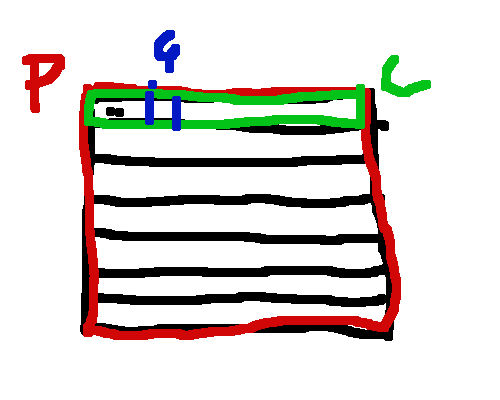
\includegraphics[scale=1.0]{images/Population_Chromosom_Gen.png}
    \caption{Gen, Chromosom und Population}
    \label{fig:population_chromosome_gene}
\end{figure}

Die \textbf{fitness} eines Chromosoms ist der Wert der Zielfunktion für den Phenotyp des Chromosoms. Also der Wert der Zielfunktion für die Parameter welche die Gene des Chromosoms representieren.
Der Ablauf eines typischen genetischen Algorithmus besteht aus 4 Schritten.

\subsection{Ablauf eines genetischen Algorithmus}
Der Ausgangspunkt eines genetischen Algorithmus ist eine Population an Chromosomen. Das erstellen dieser Population nennt man \textbf{Initialisierung}. Gewöhnlicherweise wird die initiale Population zufällig gewählt. Ein Iterationsschritt des klassischen genetischen Algorithmus besteht aus Vier Schritten \cite*{GeneticAlgorithms}.
\begin{itemize}
    \item Selektion: Aus der Population wird eine Menge an Eltern gewählt
    \item Crossover: Die Eltern werden zu einer Menge an Kindern Kindern kombiniert. Typischerweise erzeugen zwei Eltern-Chromosome ein Kind-Chromosom
    \item Mutation: Die Nachkommen werden mutiert, also zufällig verändert
    \item Evaluation: Jedem Kind wird ein fitness-Wert durch die fitness-Funktion zugewiesen
    \item Ersetzung: Die Alte Generation wird durch die neue ersetzt
\end{itemize}
Der Algorithmus terminiert wenn die vorher spezifizierte Anzahl an Generationen erreicht wurde. Alternative Terminierungskriterien sind zum Beispiel maximale Laufzeit des Algorithmus oder maximale Anzahl an Generationen ohne Verbesserung \cite*{TerminologiesAndOperators}. In Figur \ref*{fig:genetic_algorithm_flowchart} wird der beschriebene Ablauf als Flussdiagramm dargestellt.
\begin{figure}[h!]
    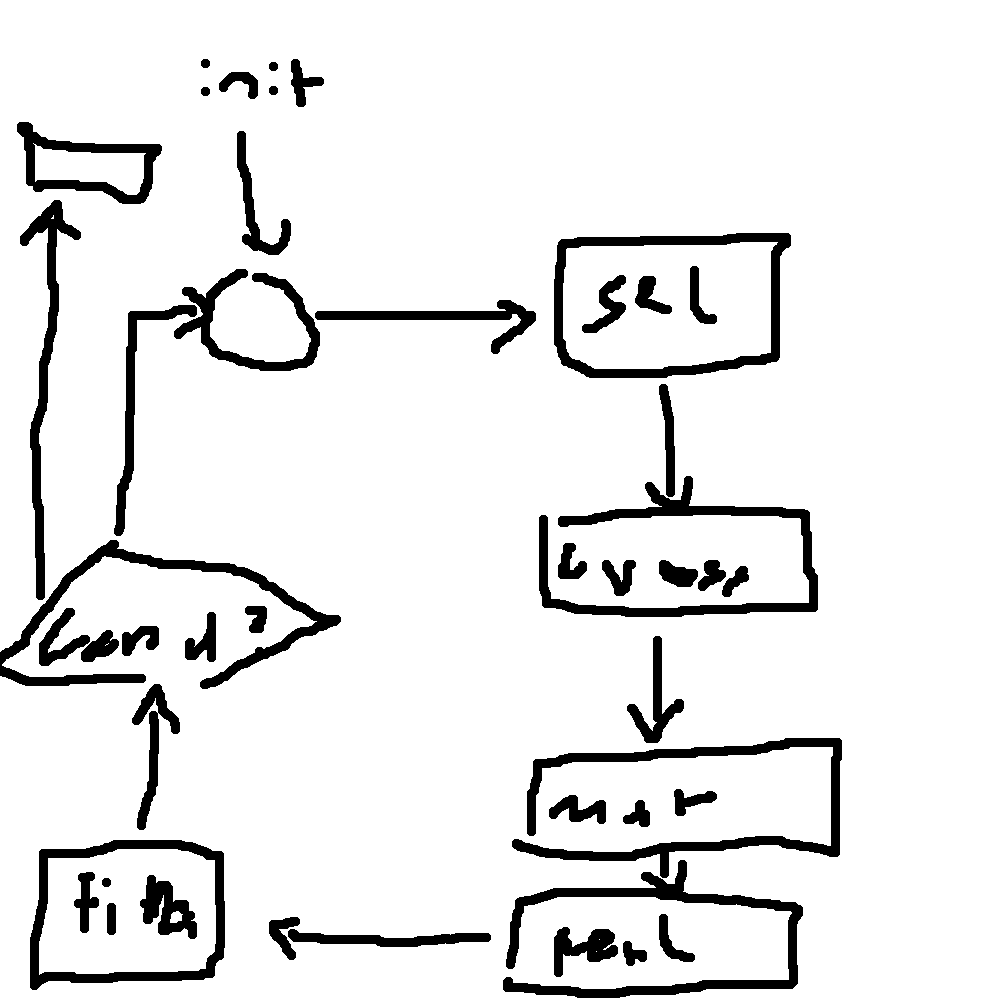
\includegraphics[scale=1.0]{images/Genetic_Algorithm_Flowchart.png}
    \caption{Flussdiagram eines genetischen Algorithmus}
    \label{fig:genetic_algorithm_flowchart}
\end{figure}


\subsection{Selektionsoperator}
Der Selektionsoperator wählt eine Menge von Eltern aus der Population, aus welchen Kinder für die nächste Generation erzeugt werden. Typischerweise hat jedes Kind-Chromosom zwei Eltern-Chromosome. Es gibt jedoch auch Crossover-Operatoren welche mit mehr als zwei Eltern arbeiten. Ganz nach der Evolutionstheorie sollen hier Chromosome mit einer höheren Fitness auch eine höhere Chance haben als Elternteil gewählt zu werden. Wie stark Chromosome mit einer höheren Fitness bevorzugt werden wird als Selektionsdruck bezeichnet. Selektionsschemata können in zwei Klassen unterteilt werden, proportionale Selektion und ordinale Selektion.~\cite*{TerminologiesAndOperators} Eine proportionale Selektion gewichtet Chromosome anhand ihrer Fitness. Ordinale Selektion gewichtet Chromosome anhand ihres Ranges. Der Selektionsdruck Bei einer proportionalen Selektion ist der Selektionsdruck hoch und es besteht das Risiko einer verfrühten Konvergenz. Denn wenn es ein Chromosom gibt, welches weitaus fitter als der Rest der Population ist wird dieses einen proportionalen Selektionsprozess dominieren und somit die genetische 
Diversität der Population senken. Andererseits führt ein geringer Selektionsdruck zu langsamer konvergenz.~\cite{TerminologiesAndOperators}
Die Auswahl des Selektionsoperators sollte also wohlüberdacht sein.

\subsubsection*{Roulette Rad Selektion}
Roulette Rad Selektion ist einer der traditionellen proportionalen Selektionsoperatoren. Stellen wir uns ein Roulette Rad vor, welches in $N$ Segmente unterteilt ist, wobei $N$ die Anzahl der Chromosome in einer Population ist. Die Länge eines Segmentes $s_i$ ist proportional zu der normalisierten Fitness des korrespondierenden Chromosoms.
\begin{equation}
    s_i = 2 \pi \cdot \frac{fitness(i)}{\sum_{j=1}^{N} fitness(j)}
\end{equation}
Nun wird das Roulette Rad gedreht und das Chromosom auf wessen Feld man landet wird in die Menge der Eltern aufgenommen. Diese Prozedur wird so oft wiederholt bis man die gewünschte Anzahl an Eltern gesammelt hat.

\subsubsection*{Zufällige Selektion}
Der zufällige Selektionsoperator ist der simpelste. Jedes Chromosom hat die gleiche Wahrscheinlichkeit in die Elternmenge aufgenommen zu werden.

\subsubsection*{Rang Selektion}
Die Rang Selektion ist eine Abwandlung der Roulette Rad Selektion. Die länge eines Segmentes ist jedoch nicht proportional zu der fitness sondern proportional zu dem Rang des Chromosoms.
\begin{equation}
    s_i = 2 \pi \cdot \frac{N - rank(i)}{\sum_{j=1}^{N} rank(j)}
\end{equation}

\subsubsection*{Elitismus}
Die Selektionsoperatoren garantieren nicht, dass die besten Chromosome ausgewählt werden. Darüber hinaus kann es vorkommen, dass die besten Chromosome durch Crossover und Mutation verschlechtert werden, sodass die Fitness der folgenden Generation geringer als die vorherige ist. Um eine Abnahme der Fitness zu verhindern kann wird Elitismus angewendet. Die n besten Chromosome einer Population, die sogenannten Eliten werden  auf jeden Fall in die nächste Generation aufgenommen ohne durch Crossover und Mutation verändert zu werden.

\subsection{Crossoveroperator}
Crossover bezeichnet das Rekombinieren von typischerweise zwei Eltern-Chromosomen zu einem Kind-Chromosom. Der vollständigkeit halber sei angeführt, dass auch Crossoveroperatoren existieren, welche  mit mehr als zwei Eltern akzeptieren oder mehr als ein Kind produzieren. In dieser Arbeit beschränken  wir uns jedoch auf Crossoveroperatoren von zwei Eltern zu einem Kind. Beim Crossover werden keine neuen Informationen in den Genpool eingeführt sondern  es werden nur die vorhandenen Gene der Eltern rekombiniert. Es folg eine Aufzählung gängiger Crossoveroperatoren.

\subsubsection*{Single Point Crossover}
Beim Single Point Crossover wird ein Cutpoint entlang der länge der Eltern gewählt. Beide Eltern werden dann an diesem Cutpoint geschnitten und das Kind-Chromosom setzt sich zusammen aus der ersten Hälfte des ersten Elternteils und der zweiten Hälfte des zweiten Elternteils.

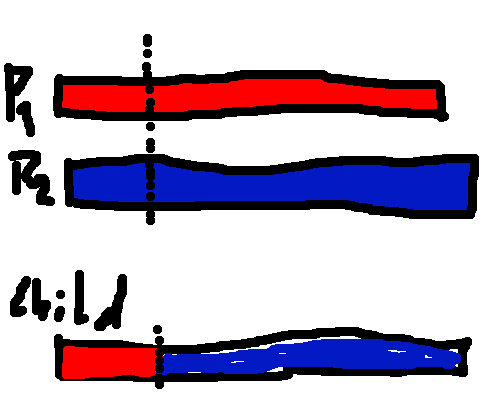
\includegraphics[scale=1.0]{images/Single_Point_Crossover.png}

\subsubsection*{N-Point Crossover}
Der N-Point Crossover ist eine Generallisierung des Single Point Crossovers. Es werden $n$ Crossover Points entlang der Länge der Eltern gewählt. Anhand dieser Crossover Points werden die Eltern in $n+1$ Segmente unterteilt. Das Kind erhält alle Segmente mit geradem Index vom ersten Elternteil und alle Segmente mit ungeradem Index vom zweiten Elternteil. Im Allgemeinen führen mehr cutpoints jedoch zu einer geringeren Effizienz  des genetischen Algorithmus.~\cite*{TerminologiesAndOperators}

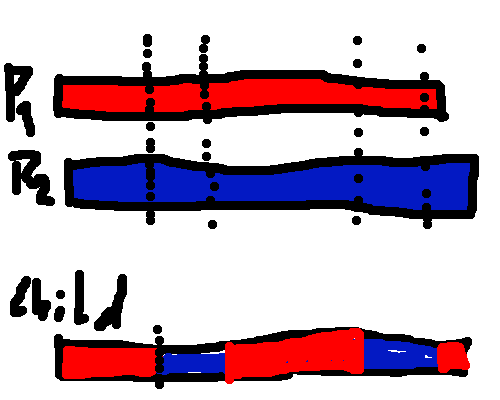
\includegraphics[scale=1.0]{images/N_Point_Crossover.png}

\subsubsection*{Uniform Crossover}
Bei einem uniformen Crossover wird eine Crossovermaske $m$ mit gleicher Länge zu den Eltern erstellt. Das Kind erhält Gene der Eltern nach dieser Crossover Maske, wobei $m_i$ angibt, von welchem Elternteil das $i$-te Gen bezogen wird. Für jedes Elternpaar wird eine neue Crossovermaske erstellt. Typischerweise gilt $P(m_i = 1) = P(m_1 = 0) = 0.5$. Die Wahrscheinlichkeit, dass ein Gen von einem Elternteil bezogen wird kann jedoch auch gewichtet werden anhand der Fitness oder Ränge, so dass $P(m_i = 0) = w$ und $P(m_i = 1) = 1 - w$

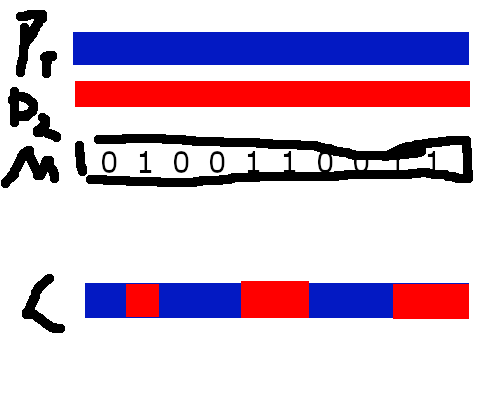
\includegraphics[scale=1.0]{images/Uniform_Crossover.png}

\subsection{Mutationsoperator}
Der Crossoverschritt verringert unweigerlich die genetische Diversität der Population. Um dem entgegenzuwirken muss es einen Mechanismus geben, welcher neues genetisches Material hinzufügt. Dieser Mechanismus ist die Mutation, welche ein Chromosom zufällig verändert.

TODO: Include Examples for Real valued GA crossover 

\subsubsection*{Mutationschance}
Die Mutationschance bestimmt wie viele Gene eines Chromosoms durch die Mutation verändert werden und wie viele Unverändert bleiben. Bei einer Mutationschance von 100\% werden alle Gene eines Chromosoms verändert  und der genetische Algorithmus ist equivalent zu einer zufälligen Suche.~\cite*{TerminologiesAndOperators}

\subsection{Ersetzen}
TODO: Ersetzen moped schmoped


Population Size
Wählt man diese Zu gering kann es zu einer verfrühten Konvergenz und somit auch einer schlechten Lösung kommen
Gleichzeitig ist die Population size ein Maßgebender Faktor in der Rechenzeit und eine zu große Population könnte 
Rechenzeit verschwenden [GAs]


Im folgenden werde ich bekannte implementationen der genetischen Operatoren eingehen und beschreiben worauf man bei der implementation achten muss

\subsection*{Mutationsoperatoren}
Random Uniform Mutation:
Random Unifor mutation 


\subsection*{Parameter eines genetischen Algorithmus}
Wie im Abschnitt [Abschnitt Label hier] erwähnt haben Metaheuristiken den Nachteil, dass sie neue Parameter einführen. Ein genetischer Algorithmus, wie er zuvor beschrieben wurde hat folgende Parameter.
\begin{enumerate}
    \item Populationsgröße
    \item Anzahl der Generationen (oder Abbruchbedingung)
    \item Mutationsfunktion und Mutationsrate
    \item Crossoverfunktion und Crossoverrate
    \item Selektionsfunktion
    \item Anzahl der Eliten
    \item Ersetzungsstrategie
\end{enumerate}
Die Belegung dieser Parameter ist keinesfalls trivial denn die Parameter beeinflussen die Konvergenzrate des Algorithmus maßgeblich. Die Populationsgröße zum Beispiel beeinflusst die globale Suchkapazität, ein größerer Wert ist hier von Vorteil. Jedoch benötigt eine große Populationi auch mehr Rechenleistung, Speicher und Zeit \cite*{TerminologiesAndOperators}. Die Mutationsrate beeinflusst ebenfalls die Konvergenzrate. Eine zu hohe Mutationsrate führt zu einer langsamen Konvergenz und einem ineffizienten Algorithmus. Eine zu niedrige Mutationsrate führt wiederum zu einer verfrühten Konvergenz und somit zu weniger optimierten Lösungen. Die Auswahl der genetischen Operatoren wirkt sich unter anderem auf die Rechenlast aus. Ein Single-Point-Crossover zum Beispiel generiert eine zufällige Zahl, und macht einen Vergleich. Die Anzahl der benötigten Zufallszahlen und Vergleiche bei einem Uniform-Crossover hingegen sind equivalent zu der Anzahl an Genen. Bei mehreren Hunderten von Genen macht sich dieser Unterschied durchaus bemerkbar.